%%%%%%%%%%%%%%%%%%%%%%%%%%%%%%%%%%%%%%%%%%%%%%%%%%%%%%%%%%%%%%%%%%%%
% Technologies and Implementation
%%%%%%%%%%%%%%%%%%%%%%%%%%%%%%%%%%%%%%%%%%%%%%%%%%%%%%%%%%%%%%%%%%%%

\chapter{Implementation}
  \label{Implementation}
The following chapter explains how the user interface is structured and which options it supports for the user, after describing the intention of this project.
\section{Motivation}
Figuring out a linear layout with certain properties by hand is a time consuming, error-prone task. This is why efforts have been made to automate this process. The discovery that SAT formulas could do this quite efficiently \cite{Bekos2015TheBE} was a big achievement.\\
Up to now the graphs had to be transformed into a textual representation in order to then be translated to a SAT instance and passed to the solver. Therefore the objective of this project was to develop an editor where a graph can be created as a drawing, then be passed to a translating routine and a solver. After receiving the solver result, the linear layout should be displayed again in a visually appealing way.\\
Furthermore it was an ambition to be able to check a graph for specific linear layouts, since randomized SAT-Solvers produce random linear layouts. Thankfully this can be easily achieved by expanding the SAT instance by clauses that lead the SAT-Solver in the desired direction. Therefore the editor needed an option to impose such constraints upon the future linear layout.\\
It was decided that the editor should be web based in order to achieve broad availability, since then nothing more than a fairly modern browser is needed.\\
\section{Graph Editor}
\begin{figure}[!h]
\begin{center}
\includegraphics[width=1\textwidth]{figures/figIndex/overviewIndex.jpg}
\caption{Overview over the user interface}
\label{img:overviewIndex}
\end{center}
\end{figure}
\subsection{Overview}
The user interface of this tool consists of three main components: the toolbar on top, the interactive graph editor in the middle and the configuration panel, where the user can specify the linear layout he or she wishes to compute.\\
\subsection{Graph Editor}
The graph editor occupies the center area of the user interface. It displays a grid by default which can be disabled.\\
\subsubsection{User Interaction}
Vertices are created by clicking on the canvas. Edges can only be created between two existing vertices, by dragging a line from the source vertex to the target. By default, double edges are forbidden but can be allowed by the user through the \textbf{tools} submenu.\\
Bends in the edges can be achieved by releasing the mouse button wherever the bend should be. In big graphs this enables a tidier drawing.\\
While every element can be placed freely on the canvas, certain positions are encouraged by clipping to the grid if visible.
The elements of a graph can be selected and then copied, cut, pasted and deleted. Edges can only be copied when duplicate edges are allowed or when at least one of the corresponding vertices is selected, too.\\
\subsubsection{Identifier of elements}
To compute the linear layout of the graph it is necessary to have a unique id for each element of the graph, so the solver can distinguish the different vertices and edges.\\
On creation every vertex and edge is assigned a label, which is displayed in the graph editor and can be changed by the user without restriction. This means that labels are not guaranteed to be unique and therefore cannot be used to identify elements.\\
Invisible for the user each vertex and edge also is assigned a tag, a feature provided by the \textit{yFiles for HTML} library. These tags cannot be changed by the user and are designed to be unique. Vertices get the next free number as a tag, edges get the tag "a-(0)-b", where a is the tag of the source vertex and b is the tag of the target vertex. The \textit{(0)} in the middle of each edge tag is necessary if the user chooses to allow duplicate edges. A duplicate edge would then be assigned the tag "a-(1)-b", ensuring the uniqueness.
\subsection{Toolbar}
On the left section of the toolbar the user can choose from submenus. The options are \textit{file}, \textit{edit}, \textit{view}, \textit{layout} as well as the licensing information of the framework and a button to toggle the visibility of the configuration panel.
\subsubsection{The file submenu}
This submenu contains means to load graphs and to save them in various formats.\\{7pt]
\begin{tabular}{p{0.05\textwidth}p{0.95\textwidth}}

\includegraphics[scale=0.6]{figures/icons/new.png} & Clears the canvas and configuration panel to create an entirely new instance\\

\includegraphics[scale=0.6]{figures/icons/download.png}& Save the current graph into the users local file system\\

\includegraphics[scale=0.6]{figures/icons/upload.png}& Load a graph from the users local file system\\

\includegraphics[scale=0.6]{figures/icons/export.png}& Export the graph to either a .png or .pdf file\\

\includegraphics[scale=0.6]{figures/icons/server.png} &Change the server to which the graph should be passed on computation. This is a feature for people who use this tool frequently and prefer to install a local copy of the server. The current server setting is displayed in the top right corner, next to the stats button. 
\end{tabular}
\subsubsection{The edit submenu}
The edit submenu gives the user options to interact with the graph.\\[7pt]
\begin{tabular}{p{0.05\textwidth}p{0.95\textwidth}}
 
\includegraphics[scale=0.6]{figures/icons/undo.png} & Undoes the last changes on the canvas\\
 
\includegraphics[scale=0.6]{figures/icons/redo.png} & Redoes the last undone changes on the canvas\\
 
\includegraphics[scale=0.6]{figures/icons/copy.png} & Copies the current selection of elements, also achievable by "ctrl + c"\\
 
\includegraphics[scale=0.6]{figures/icons/paste.png} & Pastes formerly cut or copied items to the canvas, also achievable by "ctrl + v"\\
 
\includegraphics[scale=0.6]{figures/icons/cut.png} & Cuts the current selection of elements, also achievable by "ctrl + x" \\
 
\includegraphics[scale=0.6]{figures/icons/select_all.png} & 
Selects all elements currently on the canvas, also achievable by "ctrl + a"\\

\includegraphics[scale=0.6]{figures/icons/delete_all.png} & Deletes the currently selected elements, also achievable by "del" key\\[12pt]

\includegraphics[scale=0.6]{figures/icons/marquee_all.png}  
\includegraphics[scale=0.6]{figures/icons/marquee_nodes.png}  
\includegraphics[scale=0.6]{figures/icons/marquee_edges.png} & This set of buttons changes which elements of the graph should be selected when a rectangle is dragged over the canvas. The first means all elements are selectable, the second means only vertices are selectable, the last means that only edges are selectable. This is convenient when a constraint needs to be imposed on a large group of vertices or edges.
\end{tabular}
\subsubsection{The view submenu}
Through the view submenu the user may manipulate the view of the graph.\\[7pt]
\begin{tabular}{p{0.05\textwidth}p{0.95\textwidth}}

\includegraphics[scale=0.6]{figures/icons/zoomin.png} &  Zooms into the canvas\\

\includegraphics[scale=0.6]{figures/icons/zoomout.png}&  Zooms out of the canvas\\

\includegraphics[scale=0.6]{figures/icons/focus.png} & Centers the graph on the canvas\\

\includegraphics[scale=0.6]{figures/icons/grid.png} & Toggles visibility of the grid
\end{tabular}
\subsubsection{The layout submenu}
The layout submenu provides support for different graph layout algorithms. The user can choose from the most commonly used layouts, including \textit{hierarchic}, \textit{organic}, \textit{orthogonal}, \textit{circular}, \textit{tree}, \textit{balloon} and \textit{radial} layouts.
\subsubsection{The tools submenu}
The tools submenu provides the user with additional tools to modify the graph\\
\label{toolsSub}
\begin{tabular}{p{0.05\textwidth}p{0.95\textwidth}}

\includegraphics[scale=0.6]{figures/icons/resize_nodes.png}& Toggles, whether vertices are resizable or not\\

\includegraphics[scale=0.6]{figures/icons/doubleEdges.png}& Toggles, whether duplicate edges are allowed or not\\

\includegraphics[scale=0.6]{figures/icons/stellation.png}& When no vertices are selected, this stellates every face of the graph. That means a new vertex is placed in the center each face of the graph and edges connect the new vertex to each vertex of the face (see \autoref{img:stell}). When one or more vertices are selected, the new vertex is connected to each of the selected vertex.\\

\includegraphics[scale=0.6]{figures/icons/three_stellation.png}& When less than three vertices are selected, three vertices are inserted into every face of the graph that is bounded by three edges. The new vertices are connected mutually and are also connected to the three vertices of the face (for illustration see \autoref{img:stell}). If exactly three vertices are selected this structure is inserted in between those three vertices.\\

\includegraphics[scale=0.6]{figures/icons/edgeStellation.png}& If no edge is selected, above every edge a new vertex is created, which is connected to the two end vertices of the edge. If a set of edges is selected, this only applies to those.\\
\end{tabular}
Note that the stellation for all faces of a graph only apply to \textit{planar} graphs, as there is no definition for faces in a \textit{non-planar} graph. When the user selects vertices and then applies the stellation, it works regardless of whether the graph is planar.
\begin{figure}
\begin{center}

\includegraphics[width=0.8\textwidth]{figures/figIndex/stellation.png}
\caption{Stellation of a triangular face}
\label{img:stell}
\end{center}
\end{figure}
\subsubsection{Stats}
% stats panel 
The stats panel gives information on the current graph. First of all it states how many vertices and edges the graph contains. Furthermore it provides information, whether a graph is \textit{planar}, \textit{connected}, \textit{acyclic}, a  \textit{tree} and \textit{bipartite}. The algorithms for these properties are provided by \textit{yFiles for HTML} (see \autoref{img:stats}).
\begin{figure}[!h]
\begin{center}
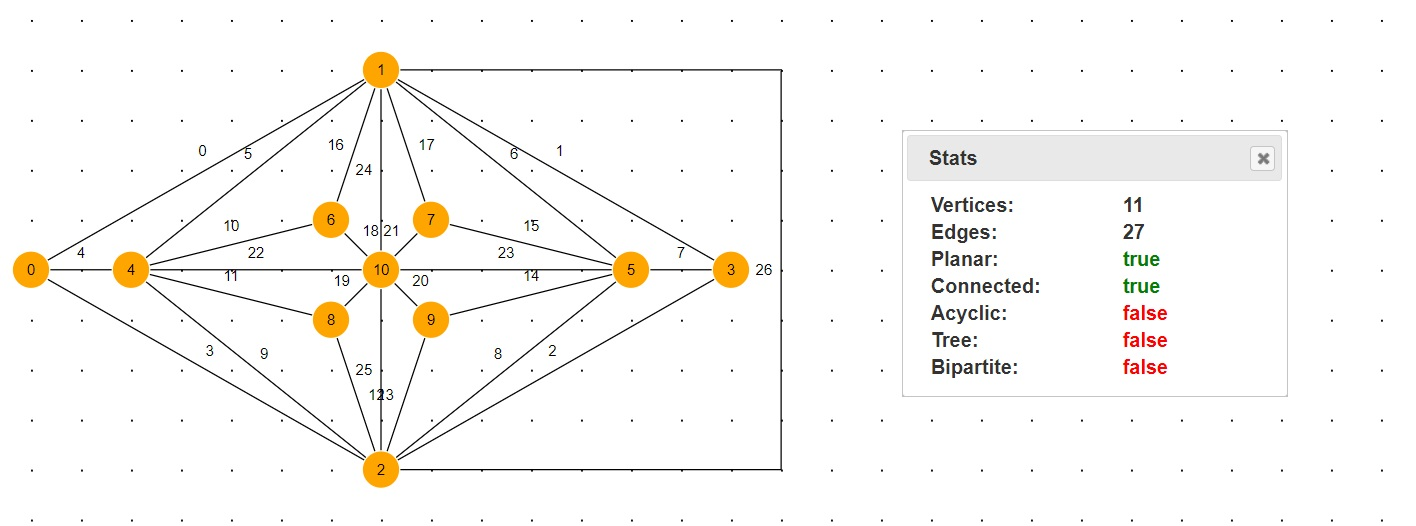
\includegraphics[width=1\textwidth]{figures/figIndex/StatsPanels.jpg}
\caption{Stats of a graph}
\label{img:stats}
\end{center}
\end{figure}
\subsubsection{Compute}
After clicking on the \textit{compute} button, a dialog opens to ask the user whether he or she would like to proceed to computing the linear layout as it is defined right now. The user then can choose to first save the graph, proceed or cancel.\\
If the computation is wished, the graph, including its constraints and page settings, is sent to the server with an ajax-request. Since the request is processed asynchronously by the server, it returns the id of the future embedding right away. This response triggers a redirection to the second page with the newly acquired id as a hash parameter.\\
If the server returns an error, the error message is displayed in a dialog and the user is not redirected.
% ajax request, transformation of data, 
\subsection{The configuration panel}
\begin{figure}[!h]
\begin{center}
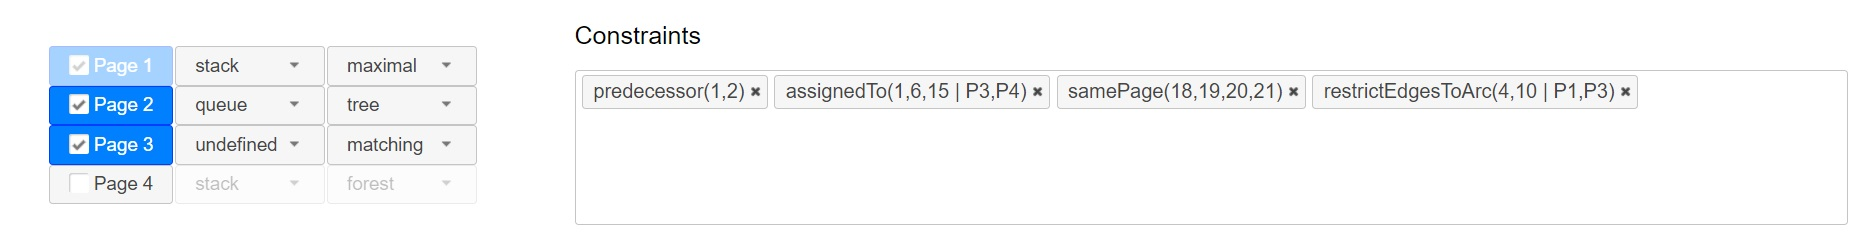
\includegraphics[width=1\textwidth]{figures/figIndex/ConfigPanel.jpg}
\caption{Configuration panel}
\label{img:confPan}
\end{center}
\end{figure}
\subsubsection{Page properties}
\label{imp_pages}
% different page constraints etc
In this panel the user can specify on how many pages the graph should be attempted to be embedded, by checking or unchecking the corresponding checkboxes.\\
The type and additional restrictions of each (checked) page can be chosen by two select menues. For types, the options \textit{undefined},\textit{stack} and \textit{queue} are available, for restrictions \textit{maximal} (meaning unrestricted), \textit{tree}, \textit{forest} or \textit{matching} (meaning a dispersable embedding) are possible.
\subsubsection{Constraints}
\label{imp_constr}
The key feature of this project is the possibility to impose constraints on the linear layout. This is needed because the SAT-Solver produces solutions to the instance on random and sometimes ît is necessary to check whether a layout with specific properties exists. For an example see \autoref{POC}.\\
The constraints are based upon an abstract class which yields a subclass for each available constraint.\\
Constraints are created via the context menu that opens whenever a selection of vertices or edges is right clicked; see the context menu in \autoref{img:constraints}.
All active constraints are saved in an array and displayed as so called tags in the \textit{Tag-It}\footnote{\url{http://aehlke.github.io/tag-it/}} plugin, which is configured so the tags can be deleted but not edited.\\
If the user chooses to delete an element from the graph the constraints corresponding to this element are also deleted, after reminding the user of this and giving the opportunity to cancel the deletion.
\begin{figure}
\begin{center}
\includegraphics[width=\textwidth]{figures/figIndex/Constraints.jpg}
\caption{The available constraints in context menues}
\label{img:constraints}
\end{center}
\end{figure}
\subsubsection{Restrict the linear order}
\label{linRestr}
To restrict the linear order of the vertices, the user can impose the following constraints:
\begin{enumerate}
\item \textbf{First in order:} When only one vertex is selected it can be set as the first node in the linear order of the linear layout.
\item \textbf{Predecessor:} With this constraint the user can specify a relative order of the vertices by defining one vertex as the predecessor of another. It implicitly also provides successorship, by reversing the predecessor relation.
\item \textbf{Consecutivity:} With this constraint two vertices can be required to be consecutive in the linear layout. It does not restrict the order of the vertices further.
\item \textbf{Partial order:} When a sequence of at least two vertices is selected, an absolute partial order of these vertices can be either required or forbidden, meaning the exact order in which the vertices have been selected, as can be seen in \autoref{img:partOrder}. If the vertices are not selected individually the order is determined by the time of creation. For easier usage the order in question is displayed in a dialog. 
\begin{figure}
\begin{center}
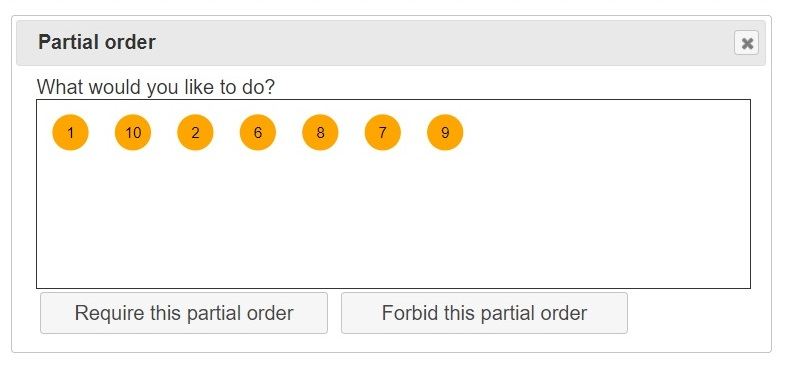
\includegraphics[width=\textwidth]{figures/figIndex/PartialOrder.jpg}
\caption{Partial order dialog}
\label{img:partOrder}
\end{center}
\end{figure}
\end{enumerate}

\subsubsection{Restrict the placement of edges}
\label{edgeRestr}
\begin{enumerate}
\item \textbf{Assign edges to certain pages:} 
When one or more edges are selected, right-clicking and selecting "Assign to.." opens a dialog, where the user can choose on which pages of the embedding these edges can be located. The set of selected edges is not necessarily on the same page, if more than one page is selected.  
\item \textbf{Assign edges to the same page:} Similar to assigning to certain pages, the user can also specify that the selected edges should be placed on the same page. 
\item \textbf{Assign edges to different pages:}
As long as the user does not select more edges than there are pages available, the user can assure that all selected edges are on pairwise different half planes of the layout by using this constraint.
\item \textbf{Not all on the same page:} For a selection of edges this constraint forbids a linear layout where all selected edges are placed on the same page of the linear layout. 
\item \textbf{Assign the edges incident to certain vertices:}
\begin{figure}
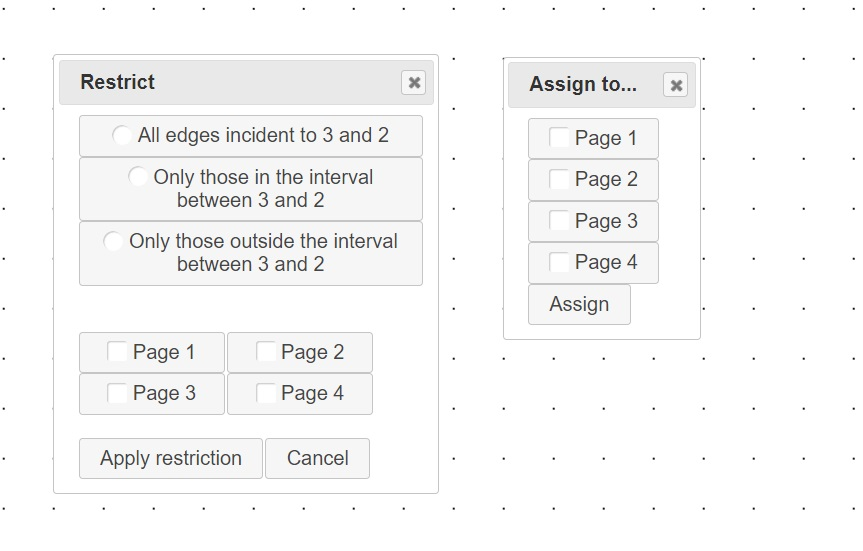
\includegraphics[width=\textwidth]{figures/figIndex/AssignAdj.jpg}
\caption{Incident edges dialog and edge assignment dialog}
\end{figure}
When the user selects two or more vertices, he or she can also constrain all edges incident to these vertices.\\
If exactly two vertices, say \textit{u} and \textit{v}, are selected, the user can choose to constrain all edges incident to these vertices or to constrain the edges that will end either in the interval between \textit{u} and \textit{v} or the interval between \textit{v} and \textit{u}. If more than two edges are selected these two latter options are not available.\\
\end{enumerate}
It is important to note that the corresponding constraints only show up if the selection is exclusively vertices, respectively edges. Otherwise the context menu would be too unwieldy to use efficiently. 
\section{Linear Layouts Viewer}
\subsection{Overview}
The viewer is structured similarly to the editor, with a toolbar on top, the viewing area in the middle and a panel on the bottom, where the imposed constraints are displayed and the appearance of the linear layout can be modified to ease its examination.
\begin{figure}[!h]
\begin{center}
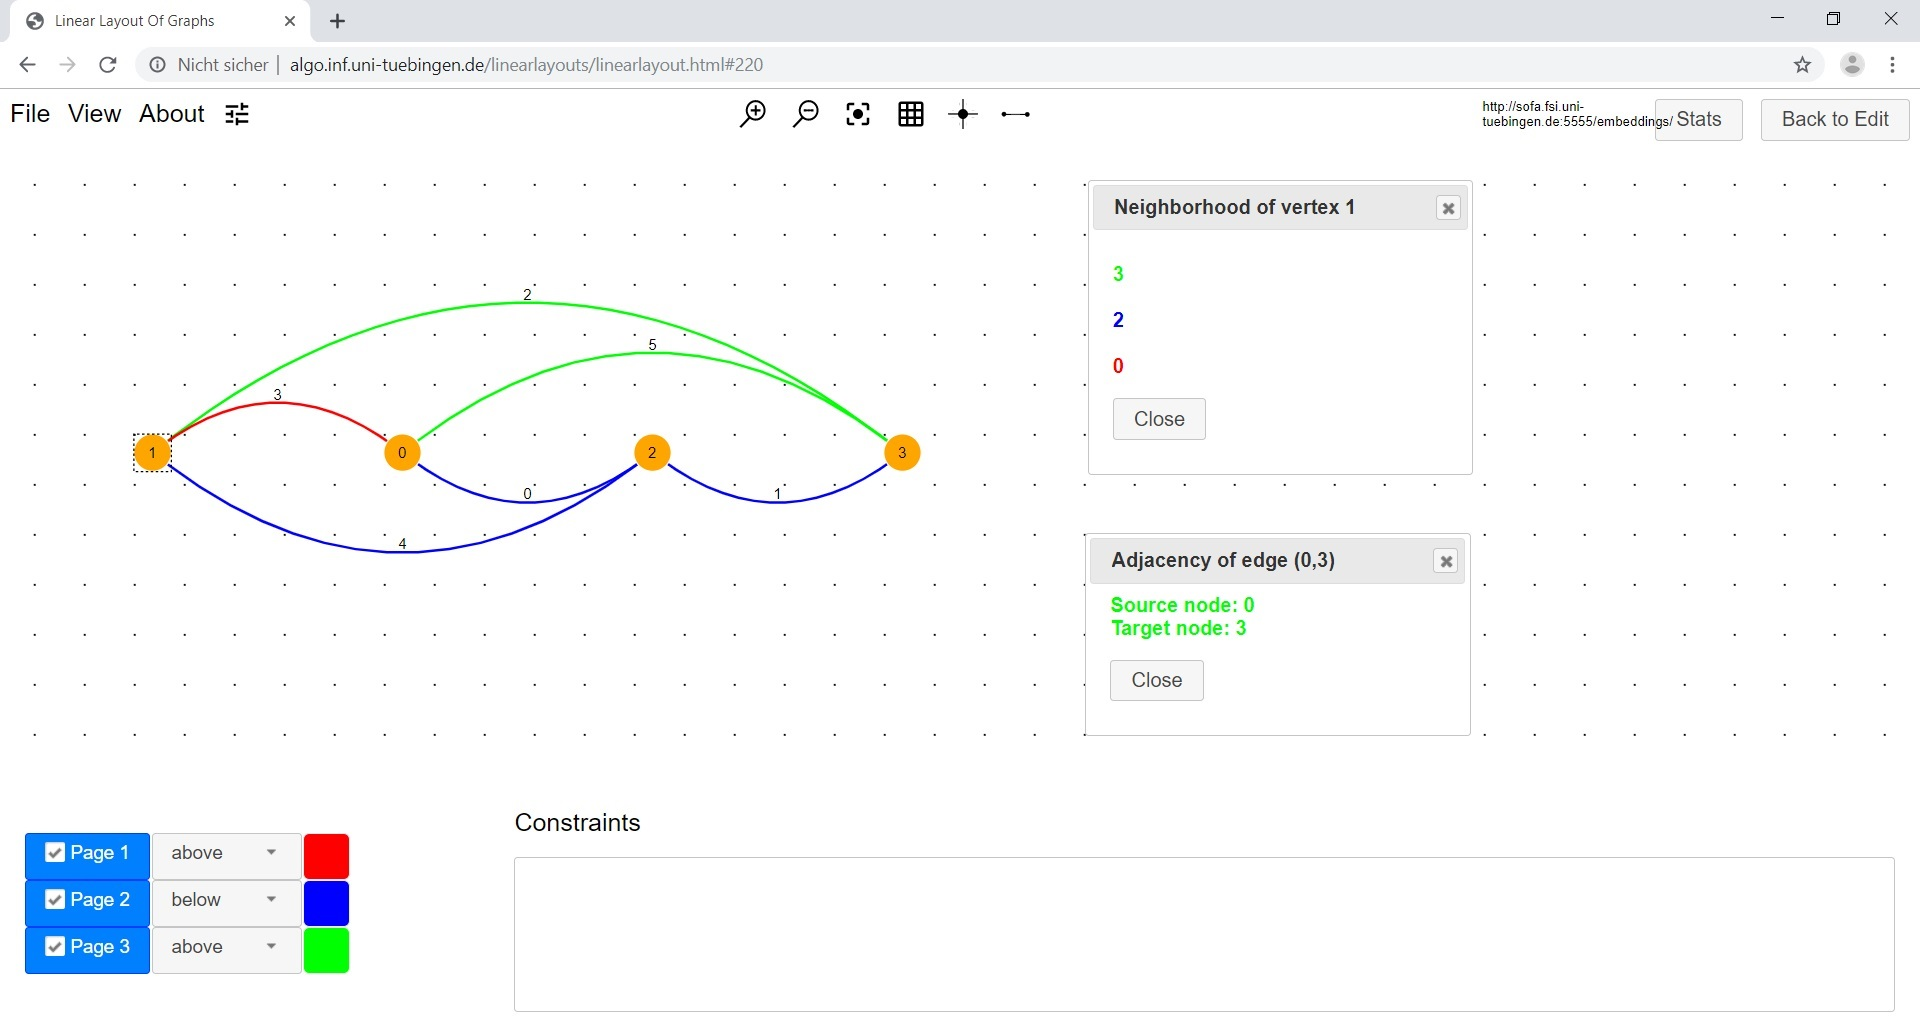
\includegraphics[width=1\textwidth]{figures/figSecond/OverviewSecond.jpg}
\caption{Overview of the viewing page}
\label{img:plzhltr}
\end{center}
\end{figure}
% how to transform graph, difficulty with arc edges, reading in constraints and pages etc, hash systems
\subsection{Linear layouts viewer}
\label{viewerOV}
% non editable but clickable
As the user accesses the second page, either directly or by redirection from the editor the url is checked for the hash parameter, where the id of the desired embedding should be located. If there is no id specified an error dialog shows up, otherwise an ajax-request is sent to the server.\\
The response is a JSON-encoded object and contains the following fields \cite{linearLayoutApi}\\[12pt]
\begin{tabular}{l p{0.7\textwidth}}
id & The id of the embedding\\
graph & The 64-byte encoded graph that was sent to the server\\
pages & The pages of the embedding as JSON objects in a list, each with the attributes \textit{id}, \textit{type} and \textit{layout}\\
constraints & S list of constraints as JSON objects. Each constraint object has the attributes "type", "modifier" and "arguments".\\
status & A string, either "IN\_PROGRESS" or "FINISHED", determining if the server finished the computation of the embedding or not\\
vertex order & A list of strings, where each string is the tag of a vertex. This list is ordered like the vertices need to be ordered along the spine of the linear layout\\
satisfiable & A boolean, determining whether the graph was embeddable as proposed\\
rawSolverResult & The result as returned by the SAT-Solver\\
created & a timestamp in string form, e.g. \textit{'2019-06-25T09:50:13.122499+00:00'}
\end{tabular}\\[12pt]
After the client received the response from the server it checks the status of the response. As long as the status is "IN\_PROGRESS", another request is sent after 5 seconds. During this waiting time the user can cancel the computation and return to editing the graph (see \autoref{Waiting}). Once the computation is finished the status changes to "FINISHED". Then as the second step the website checks if the graph was embeddable in the way it was defined, which is stated in the field \textit{satisfiable}. If it is not embeddable a dialog shows up, allowing the user to go back to editing the graph (see \autoref{NoEmb}).\\
\begin{figure}
\begin{center}
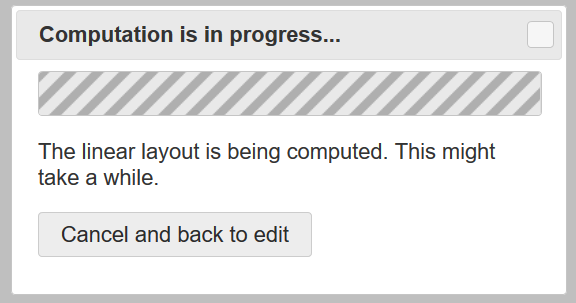
\includegraphics[width=0.5\textwidth]{figures/figSecond/waittime.png}
\caption{Waiting time dialog}
\label{Waiting}
\end{center}
\end{figure}
\begin{figure}
\begin{center}

\includegraphics[width=\textwidth]{figures/figSecond/NotEmbeddable.jpg}
\caption{Dialog when a graph is not embeddable as desired}
\label{NoEmb}
\end{center}
\end{figure}
\noindent If it was indeed embeddable the website proceeds to modify the graph to display the linear layout in the following steps:
\begin{enumerate}
\item The graph is decoded and loaded into the viewer
\item The vertices are ordered according to the "vertex order" field of the response
\item The edges are partitioned into sets representing each half plane of the graph, according to the \textit{assignment} field.
\item Each edge is assigned the "Arc Edge Style" provided by \textit{yFiles for HTML}. 
\item For each set representing a page of the embedding, all edges in this set get assigned a color. The sets of edges are positioned alternatingly above and below the spine by changing the height attribute of the affected arcs.\\
\end{enumerate}
\subsection{Toolbar}
The toolbar of the viewing page is structured similarly to the editing page, though the options were adjusted to fit the requirements.\\
% mostly the same as before but less
The file submenu does no longer allow to load graphML files but still provides the saving and exporting options.\\[12pt]
The view submenu still has the same options as before, so the user can zoom in and out, center the graph on the screen and toggle the visibility of the grid.\\
Additionally, it also provides the user with means to examine the vertex neighborhood and edge adjacencies in the graph.\\
The \textit{about} dialog can still be accessed on the second page and similar to the first page the user can hide the configuration panel to enlarge the graph viewing area. The \textit{stats} button is in the same place as before, too.\\
Where the \textit{computation} button was before there is now a \textit{back to edit} button that allows the user to either edit the original layout or the linear layout through redirecting him or her back to the editor. This redirection is explained later.
\subsubsection{Neighborhood and adjacency dialogs}
\label{NandA}
The \textit{vertex neighborhood} and the \textit{edge adjacency} buttons in the \textbf{view} tab of the toolbar each open a dialog. \\
\begin{itemize}
\item The \textbf{vertex neighborhood} dialog holds information about the vertex that is currently selected and is only updated as a different, single vertex is selected. It lists the neighboring vertices and displays them in the color of the edge that connects the selected vertex to its neighbor.
\item The \textbf{edge adjacency} dialog tells the user what is the source and end vertex of the edge currently selected. Similar to the \textit{vertex neighborhood} it is only updated, when another edge is selected.
\end{itemize}
These dialogs proved to be useful to observe patterns in large graphs, since tracking edges turned out to be cumbersome.
\begin{figure}[!h]
\begin{center}
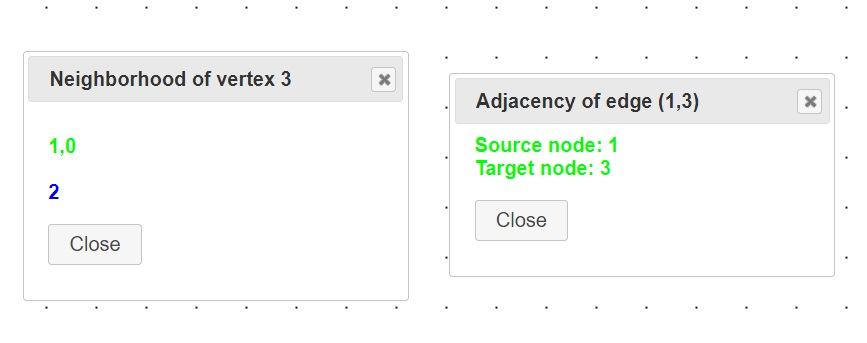
\includegraphics[width=1\textwidth]{figures/figSecond/NeighborAdjac.jpg}
\caption{Neighborhood and Adjacency}
\label{img:plzhltr}
\end{center}
\end{figure}

\subsubsection{Returning to edit the graph}
\label{BtoEdit}
When the \textit{Return to edit} button is clicked a dialog opens. The user can choose to either edit the linear layout or the original embedding of the graph. After choosing, a redirection back to the editing page is triggered.
The correct redirection is obtained again by adding a hash parameter to the url. If the user chooses to edit the original layout, the url is extended by "\#or" and the id of the graph otherwise it is "\#ll" followed by the id. That way a user can also access both layouts later on and even bookmark them.\\
The editing page, recognizing if there is a hash parameter set, sends an ajax-request to the server similar to the viewing page. If the user wishes to edit the linear layout the same processes as described in \autoref{viewerOV} are triggered. When the original embedding is to be edited, the graph is loaded to the editor. The edges still get colored in the respective page color, in order to make examination easier, otherwise the graph remains unchanged.\\
% displaying graph, hash system
\subsection{The configuration panel}
\subsubsection{Constraints}
In the bottom part of the page, the constraints defined in the creation of the layout are displayed in a similar fashion to the editing page, except that the user cannot delete a constraint.
\subsubsection{Page representation}
For easier observation of the embedding, the graphs representation can be modified. Each page of the embedding can be hidden by unchecking the corresponding checkbox. Furthermore the position and color of each set of edges can be changed, the first by selecting either \textit{above} or \textit{below} in a select menu and the latter with the \textit{Colorpick} plugin\footnote{https://github.com/philzet/ColorPick.js}.
\begin{figure}[!h]
\begin{center}
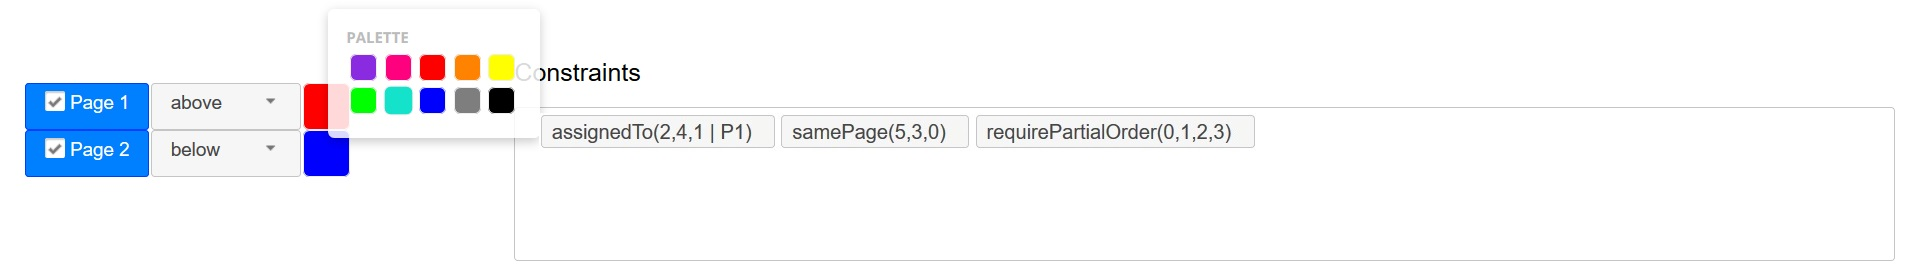
\includegraphics[width=1\textwidth]{figures/figSecond/ConfigPanel.jpg}
\caption{Pages and Constraints Panel}
\label{img:plzhltr}
\end{center}
\end{figure}

\clearpage
